\documentclass[10pt,conference,compsoc]{IEEEtran}
\usepackage[utf8]{inputenc}
\usepackage{graphicx}
\usepackage[nocompress]{cite}

% Title Page
\title{Probe or Wait: Handling tail losses using Multipath TCP}

\author{\IEEEauthorblockN{Kiran~Yedugundla, Per~Hurtig, Anna~Brunstrom}
\IEEEauthorblockA{Dept. of Computer Science, Karlstad University, Karlstad, Sweden}}


\begin{document}
\maketitle

\begin{abstract}
Packet losses are known to affect the performance of latency sensitive applications in the Internet such as media streaming and gaming. Transport protocols recover from packet loss in order to provide reliable end to end communication and improving the quality of user experience. The efficiency of loss recovery greatly influences the completion time of flows. In this paper we focus on the state of the art loss recovery mechanisms for TCP and Multipath TCP. We use controlled tail loss scenarios to evaluate the performance of loss recovery mechanisms by calculating the burst completion time for each scenario. Based on the observations, we propose an enhancement to the tail loss recovery in Multipath TCP to improve the loss recovery time. Our experiment results show end to end latency performance improvement in controlled scenarios by reducing the burst completion time. 
\end{abstract}

\section{Introduction}


Multipath TCP~(MPTCP) is an experimental standard proposed as an extension to TCP~\cite{rfc6824}. It allows devices with multiple interfaces to transmit data simultaneously on both interfaces, thereby improving the throughput of end-to-end connections. Using MPTCP, a connection can have multiple TCP subflows using different interfaces on different routes. Each TCP subflow imparts the functional behavior of a standard TCP flow. 

TCP has two mechanisms for detecting and recovering from packet losses: Fast Retransmit (FR) and Retransmission Timeout~(RTO)~\cite{Flach:2013}. Fast retransmit is triggered on receipt of a predecided number of duplicate acknowledgements, considering it as a loss indication. In case of RTO, a sender waits for the packet loss to trigger a timeout before retransmitting that packet. During timeout, the sender cannot send any packets, but with FR the out-of-order packets are presumed lost upon receiving duplicate acknowledgements. The sender can start retransmission without waiting for timeout. For flows where there are sufficiently many packets to be transferred, FR is quicker than RTO in detecting and recovering packet losses. Fast retransmit coupled with fast recovery can send data outstanding whene there is enough data to send in long flows. On the other hand, shorter flows have to depend on RTO for packet loss detection and recovery, thus incurring more latency. A single packet loss in a short flow may take many RTTs to detect and recover. This scenario is also applicable to the packets at the end of the flow (or tail), in a long flow. Although, RTO is reliable, even in tail loss recovery, it is not efficient in terms of recovery completion time. 

 MPTCP connections start with one TCP flow to send data over, and may add more flows to the connection if configured to. MPTCP uses a connection level congestion window as well as subflow level congestion windows for each subflow. Data is split across the flows and each data packet is scheduled on one of the subflows based on minimum RTT. Packet losses in each subflow are detected and recovered in a similar fashion as that of TCP. Loss recovery can be conducted at different levels: the MPTCP connection level (meta level) and at subflow level. If the recovery is handled at meta level, a lost packet may be rescheduled and retransmitted on the available subflow with the lowest RTT. If recovery is handled at the subflow level, the packet may be retransmitted on the same subflow. An important part of MPTCP packet loss recovery process is to follow the TCP semantics and retransmit lost packets on the initial path of transfer. However, the MPTCP standard does not restrict on, how the loss recovery should happen in the implementation and which subflow should retransmit the lost packets.


TCP Loss Probe (TLP)~\cite{Flach:2013} is a mechanism to detect and recover from tail losses by employing a loss probe packet for a timeout shorter than the RTO. Probe timeout enables short flows to recover packet loss at the tail, by triggering FR. It assumes other algorithms such as Early Retransmit~(ER)\cite{rfc5827} and Forward Acknowledgement~(FACK)~\cite{FACK} threshold based recovery are enabled. TLP is available in Linux kernel and enabled by default. Further evaluations in~\cite{Rajiullah:2015}, showed that TLP provides significant reductions in latency for short flows with one to n-degree tail losses. 

In this paper, we analyze the retransmission behavior of MPTCP in selected tail loss cases to identify the scope for improvement. We propose a change in the retransmission strategy of MPTCP to improve the latency performance. We provide related research on MPTCP retransmission in section~\ref{relwork}, and the experimental setup in section~\ref{exsetup}. We discuss observations from the experiments in section~\ref{disc}. Based on the observations, we propose an improvement to the current Linux implementation of TLP for MPTCP in section~\ref{impr}. In section~\ref{eval}, we provide an evaluation of the proposed TLP for MPTCP mechanism and conclude the paper in section~\ref{conc}.
 
\section{Background and Related Work}\label{relwork}

Retransmission schemes are of significant importance in achieving low flow completion time. Several research studies has led to improved retransmission strategies for TCP. The current Linux TCP implementation provides room for improvement in several packet loss scenarios. 

In a TCP flow, sequence numbers are used to identify lost packets and retransmit them. MPTCP uses two levels of sequence numbers to support efficient data transfer, namely data sequence and TCP sequence. Data sequence is for the end-to-end data transfer and TCP sequence number is for individual flow data sequence similar to TCP. There is an association between data sequence number and TCP sequence number within a subflow.  A loss occurring in an individual TCP flow corresponds to a loss in end-to-end data. Multipath TCP, as an extension of TCP, uses the basics of TCP retransmission. However, the interaction with two levels makes the problem of retransmission more challenging than in TCP. The dual sequence numbering enables MPTCP to respond to loss of packets by retransmitting the lost packets on an alternate path.  

The Linux implementation of MPTCP uses a set of retransmission heuristics to handle retransmissions. The data outstanding on a timed out subflow should be rescheduled for transmission on a different subflow using timeout as the indicator. Fast retransmit on a subflow will not trigger retransmission on another subflow. The target devices of MPTCP contain a degree of asymmetry in their interface characteristics such as 3G or 4G vs WLAN, leading to flows with different delay characteristics. Authors in~\cite{fuso}, try to exploit the path diversity by quickly retransmitting on the fastest paths. Quick retransmission comes with a cost of redundant packets as each individual TCP flow should retransmit always to follow TCP semantics. MPTCP standard suggests a more conservative approach. MPTCP is designed to exploit the multiple interfaces and often one or more of these could be wireless with completely different characteristics than that of wired interfaces. Authors in~\cite{Shin} argue that the calculation RTO for MPTCP flows should include the interface characteristics to improve loss recovery time. 


%\subsection{Scope}\label{scope}

This paper analyzes the performance of state of the art loss recovery mechanism of MPTCP and presents a case for improvement in the tail loss scenario. 
For understanding the loss recovery and retransmission policies in MPTCP Linux implementation version 0.91, we consider several specific cases of tail losses.  
We use the standard settings of the Linux kernel to understand the performance for various cases of tail loss and its recovery.
The Linux implementation of TCP is considered as the baseline TCP retransmission for implementation flexibility and availability of TLP support.

\section{Experimental Setup}\label{exsetup}

Experiments use the CORE emulation platform~\cite{CORE} with a simple topology as depicted in Figure~\ref{fig1}
with client node connected to two wireless interfaces 3G or 4G and WLAN and server node connected to a wired router.
CORE emulates the Linux networking stack in each node of the topology by using lightweight virtualization technique known as Linux network namespaces.
Characteristics of the connection setup and assumptions about the parameters are provided in Table~\ref{tab1}.
The parameters are chosen to be close to real values of bandwidth and delay of respective technologies.
There is no attempt in this study to focus on the effect of link detailed characteristics in retransmission performance.

 
\begin{figure}[!ht]
\begin{center}
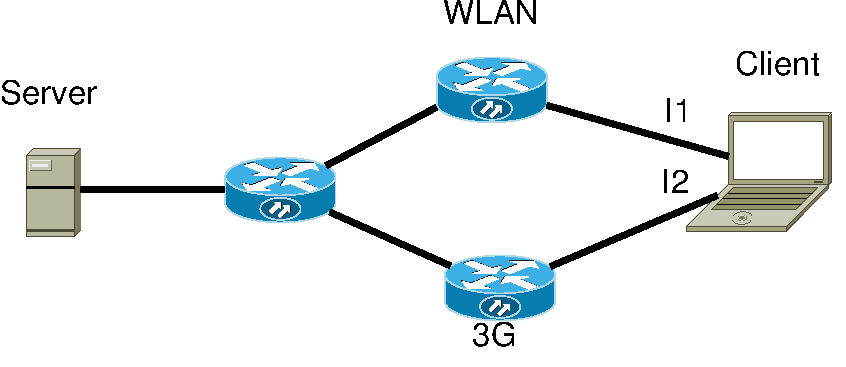
\includegraphics[angle=0, width=0.45\textwidth]{images/fortest.pdf}
\caption{Topology used for Emulation}\label{fig1}
\end{center}
\end{figure}
\begin{center}

\begin{table}
\resizebox{0.45\textwidth}{!}{\begin{minipage}{0.45\textwidth}
\small
\begin{center}
\begin{tabular}{|c|cccccccccc|}
      \hline
      
      \multicolumn{1}{c}{} & & \\[\dimexpr-\normalbaselineskip-\arrayrulewidth]
      \textbf{Burst Size} & \multicolumn{10}{c|}{80 Packets} \\
      \hline
      \textbf{Separation Time} & \multicolumn{10}{c|}{2s} \\
      \hline

      \textbf{RTT} & \multicolumn{10}{c|}{20ms-120ms(3G/4G/WLAN)}  \\
      \hline 	
      \textbf{Bandwidth} & \multicolumn{10}{c|}{54Mbps(3G/4G/WLAN)}  \\
      \hline
      \textbf{Loss Model} & \multicolumn{10}{c|}{Deterministic}\\
      \hline
      	
\end{tabular}
\caption{Emulation parameters}\label{tab1}
\end{center}
\end{minipage}}
\end{table}
\end{center}


\subsection{Testing retransmission with deterministic loss patterns}
In order to understand the retransmission behavior of the Linux MPTCP implementation and to reproduce the observed retransmissions, we use a deterministic drop pattern.
Losses are generated by associating netem with corresponding interfaces and dropping select packets. This process is simplified by using the KAUNetem tool~\cite{Garcia2016}, which allows experimenter to e.g., drop packets based on their positions in a flow. MPTCP connection starts with a single TCP subflow and subsequently, one or more subflows are added following an agreement between the client and the server. So one has to wait both in time and packets for the second subflow establishment. We send two bursts of 80 packets each and drop tail packets at one of the interfaces. This is to ensure that the necessary and sufficient conditions for probe triggering are met and tail loss probe is generated on that
subflow. Three test cases are evaluated with one packet tail loss, two packet tail loss and one packet along with probe~(in TLP) or retransmission~(in RTO) loss. 

In Linux, TCP retransmission features are controlled by a sysctl setting tcp.early.retrans. It has 5 possible values ranging from 0 to 4 with 3 being the Linux default. The default setting value enables both
ER and TLP. TCP in other operating systems might not use ER and TLP. We use RTO to refer to a sysctl setting of 0 and TLP to refer to a sysctl setting of 3 throughout the paper.
In Linux, disabling ER and TLP gives the performance of RTO. In Linux default TCP, enabling delayed ER gives the combined performance of RTO, delayed ER and TLP.
In RTO, probe loss scenario is equivalent to losing the retransmitted packet.

The setup has server and client with Linux supporting MPTCP running on them. Client has two wireless interfaces with one way delay on each interface ranging from 20ms to 120ms. We consider 5 scenarios with delay pairings 20ms-20ms, 20ms-30ms, 20ms-120ms, 30ms-20ms, 120ms-20ms to understand the effect of delay difference in the performance as shown in Table~\ref{tab1}. These scenarios are chosen to evaluate the effect of symmetry, mild asymmetry and higher asymmetry in link delays. For each experiment trail, we send two bursts of data from server to client, each burst containing 80 packets. First burst allows the MPTCP connection to be setup taking in to account that second flow is added after some time and packets. We calculate the burst completion time for second burst that has specified tail losses.

\section{Observations and Discussion}\label{disc}
This section provides the performance analysis of TCP and MPTCP for the considered cases of single packet tail loss, retransmission or probe loss and two packet 
tail loss.

\subsection{TCP}
Retransmission behavior of TCP provides a base case for MPTCP performance as each individual MPTCP subflow is a TCP flow in itself. Our analysis
starts with the results using TCP and compare it with that of the MPTCP. Figures ~\ref{t1p},~\ref{t2p},~\ref{t1pp} represent the comparison of TCP 
burst completion times. Path asymmetry is irrelevant in this case as the TCP uses single path.

In the case of single packet tail loss, there is no difference in burst completion times of RTO and TLP settings. The retransmission
timeout and the probe timeout are same as there is only one outstanding packet. This is a special case in TLP
specification that adds 200ms to PTO accommodating the case of delayed ACK. TLP implementation in Linux accounts
for the delayed ACK and waits 200ms before sending probe. The minimum of PTO and RTO is considered for PTO.

Hence retransmission timeout is the mode of loss recovery in both RTO and TLP. This can be avoided by tuning
the ACKs as discussed in~\cite{Rajiullah:2015}. In the case of two packet tail loss, TLP performs better than RTO as it employs a combination of TLP and ER to recover from losses. 
If the probe or retransmission is lost, then TLP still performs better than RTO as it waits for one probe timeout and one RTO instead of two RTOs.

\begin{figure}[!ht]
\begin{center}
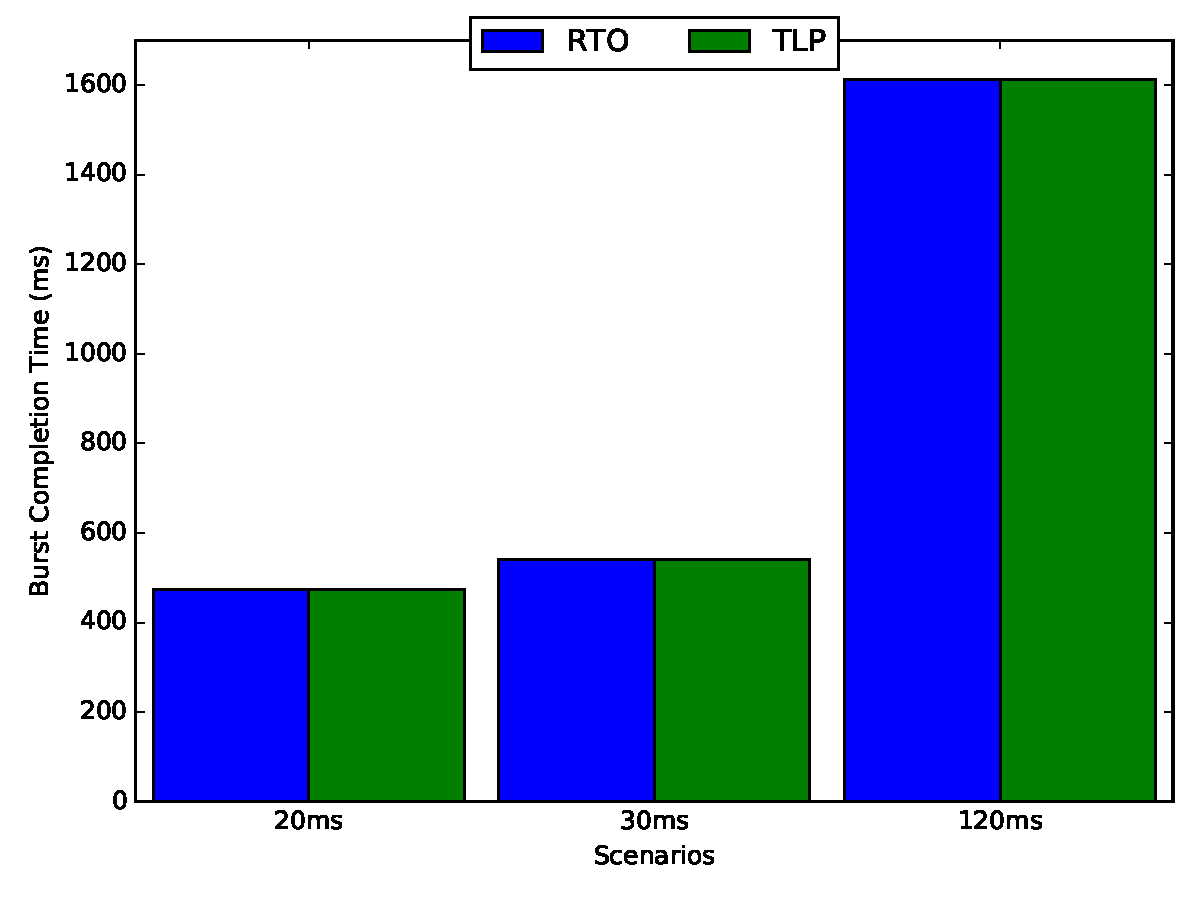
\includegraphics[angle=0, width=0.46\textwidth,natwidth=578.16,natheight=433.62]{plots/T1P.pdf}
\caption{Single packet tail loss using TCP}\label{t1p}
\end{center}
\end{figure}



\begin{figure}[!ht]
\begin{center}
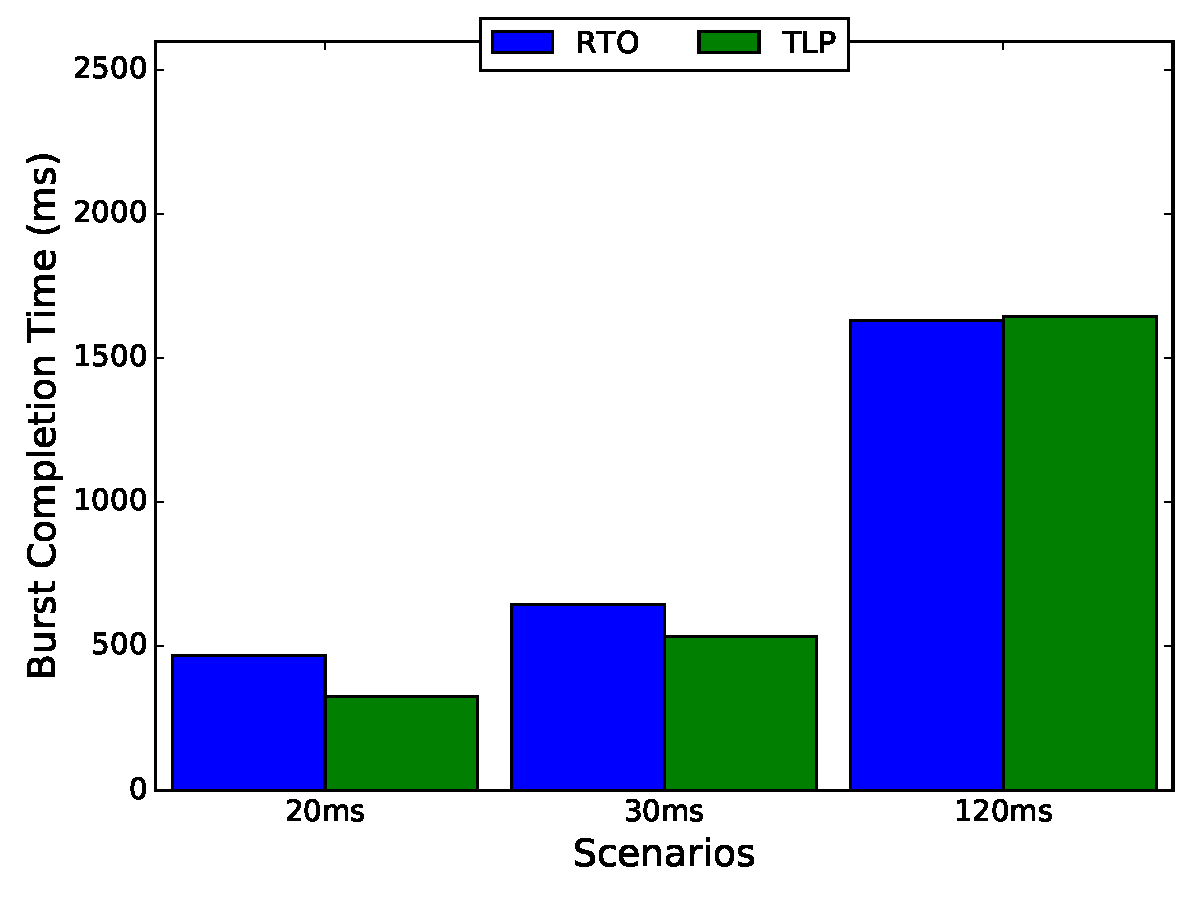
\includegraphics[angle=0, width=0.46\textwidth,natwidth=578.16,natheight=433.62]{plots/T2P.pdf}
\caption{Two packet tail loss using TCP}\label{t2p}
\end{center}
\end{figure}


\begin{figure}[!ht]
\begin{center}
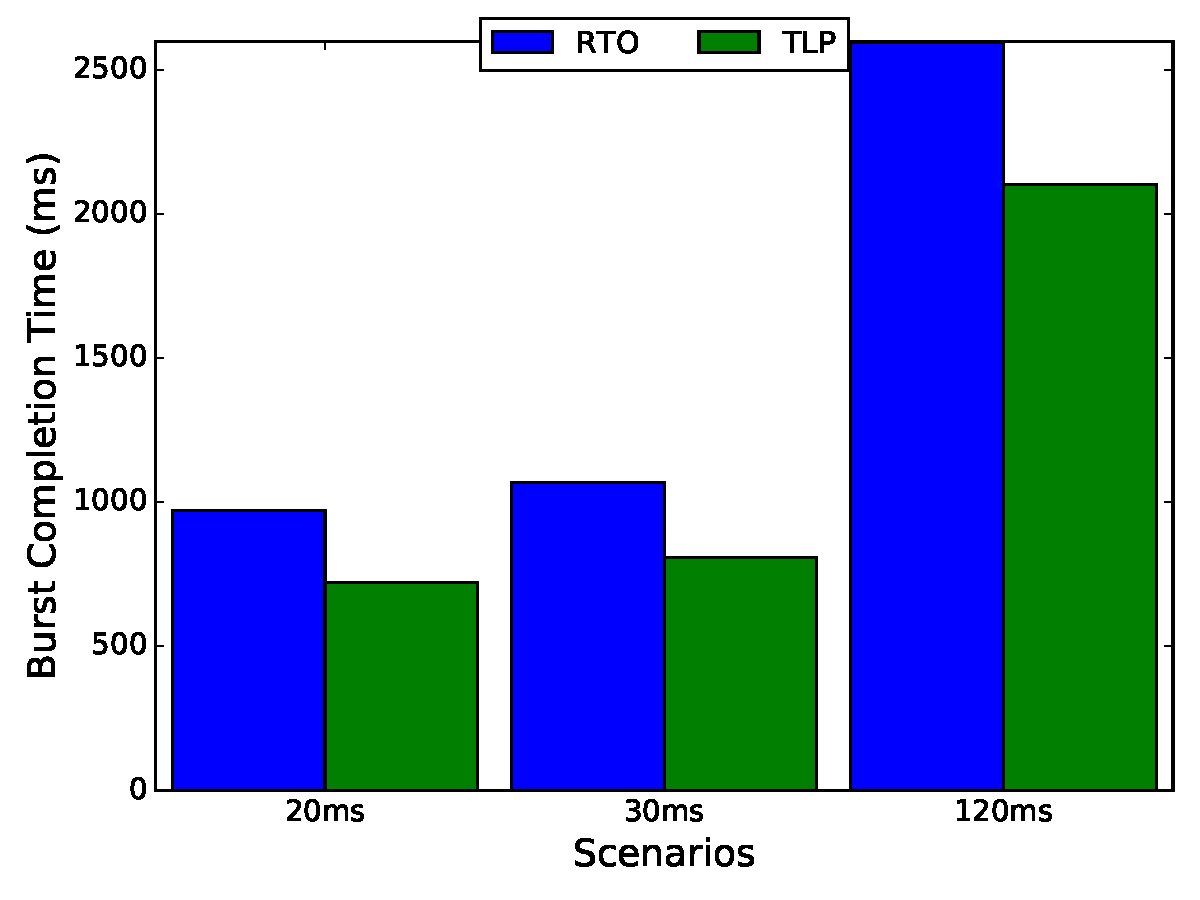
\includegraphics[angle=0, width=0.46\textwidth, natwidth=578.16,natheight=433.62]{plots/T1PP.pdf}
\caption{Single packet tail loss together with retransmission loss using TCP}\label{t1pp}
\end{center}
\end{figure}

\subsection{MPTCP}


The expected retransmission behavior of MPTCP for RTO and Linux default settings is shown 
in~\ref{timing1P},~\ref{timing1PP} and ~\ref{timing2P}. The actual pattern might differ in cases,
where the RTT is larger than 200ms. 

\begin{figure}[!ht]
\begin{center}
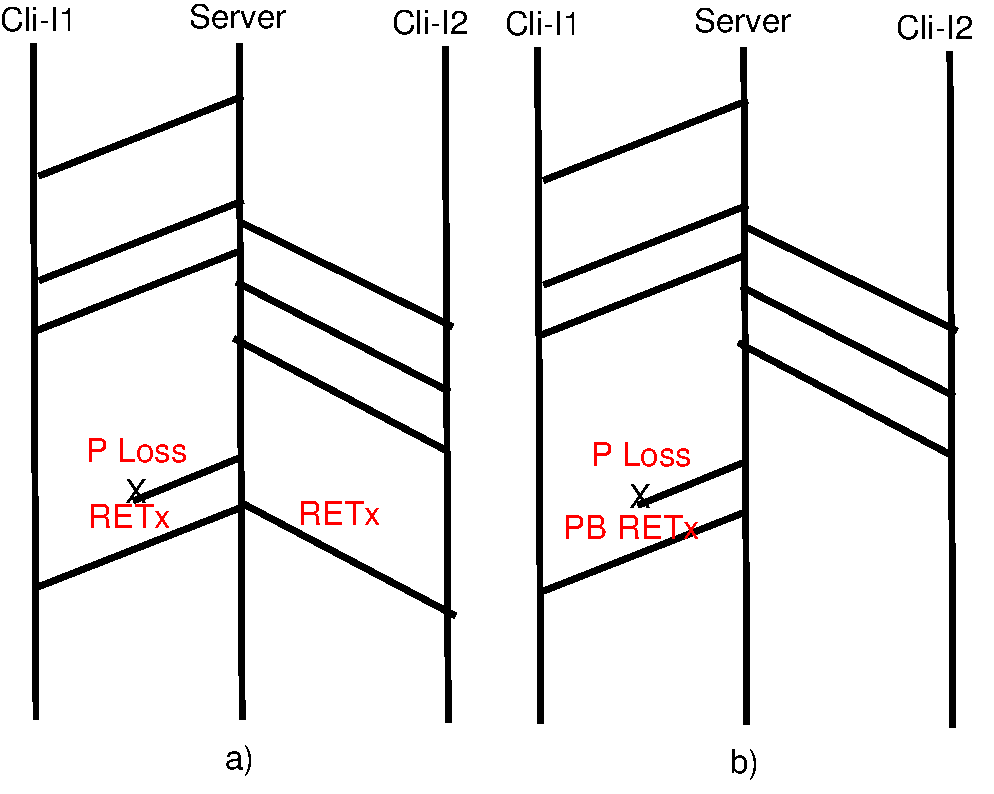
\includegraphics[angle=0, width=0.45\textwidth, natwidth=610, natheight=400]{images/timing1P.pdf}
\end{center}
\caption{Timing diagram of MPTCP behavior with one packet tail loss a) RTO b) TLP}\label{timing1P}
\end{figure}

\begin{figure}[!ht]
\begin{center}
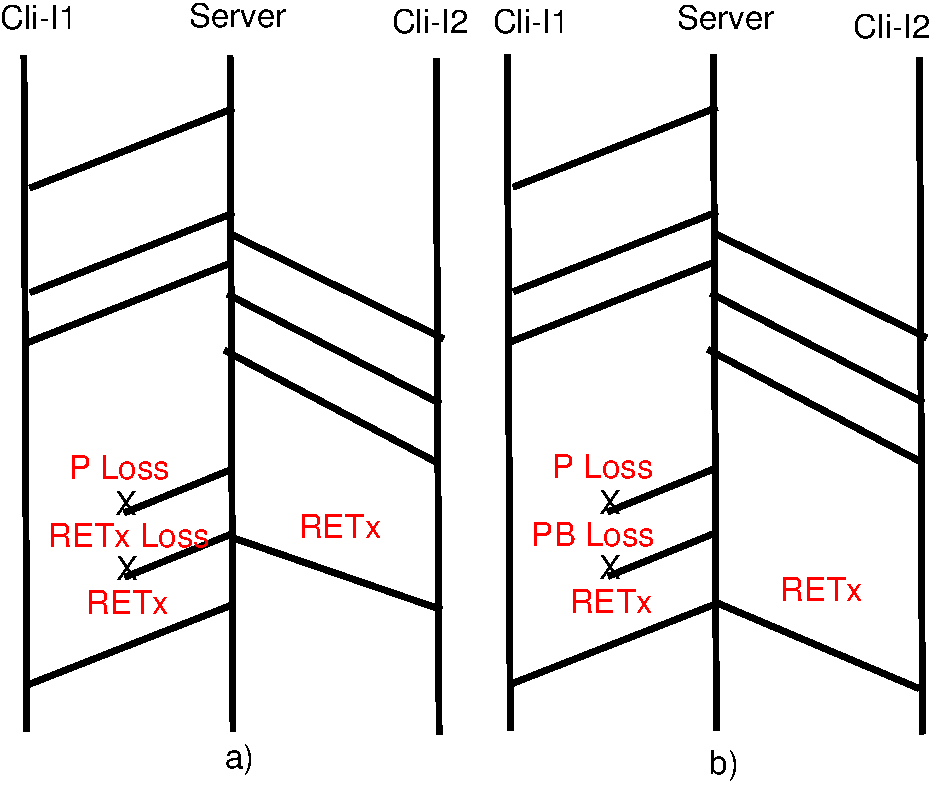
\includegraphics[angle=0, width=0.45\textwidth, natwidth=610, natheight=400]{images/timing1PP.pdf}
\end{center}
\caption{Timing diagram of MPTCP behavior with one packet and next probe loss a) RTO b) TLP}\label{timing1PP}
\end{figure}

\begin{figure}[!ht]
\begin{center}
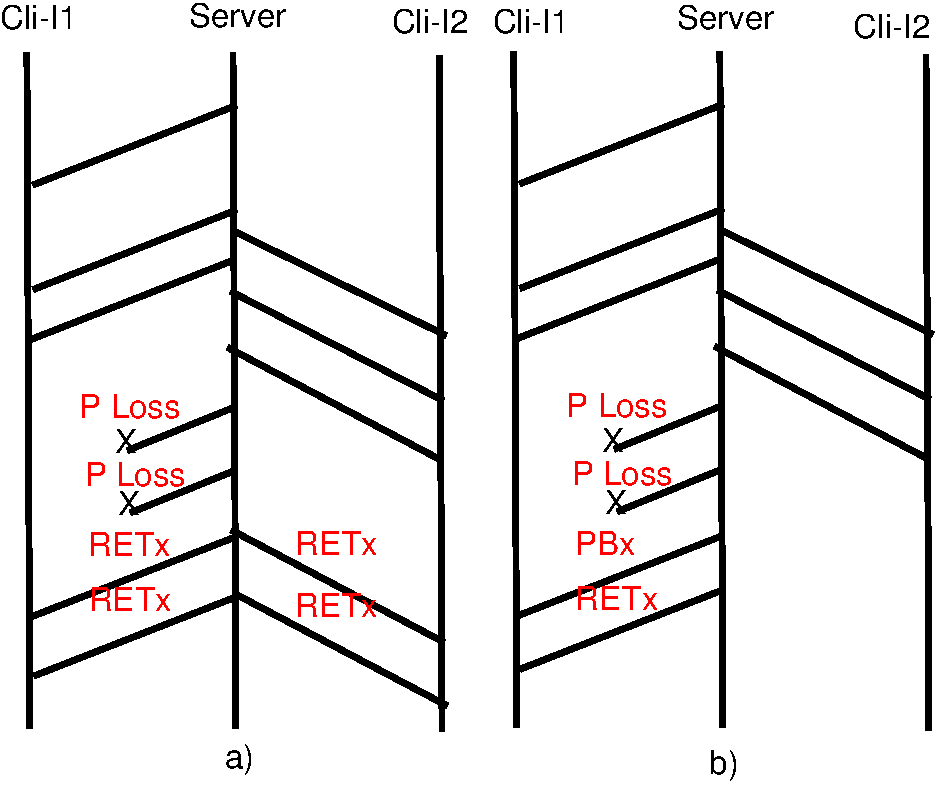
\includegraphics[angle=0, width=0.45\textwidth, natwidth=610, natheight=400]{images/timing2P.pdf}
\end{center}
\caption{Timing diagram of MPTCP behavior with two packet tail loss a) RTO b) TLP}\label{timing2P}
\end{figure}



Experiments performed on CORE emulator with the setup mentioned in section~\ref{exsetup}. MPTCP is sensitive to path asymmetry in general due to the default scheduler being shortest RTT based scheduler.

The burst completion times on single packet tail loss calculated for each delay configuration and retransmission 
setting is depicted in Figure~\ref{1p}. There is no difference in performance of RTO and TLP. 

\begin{figure}[!ht]
\begin{center}
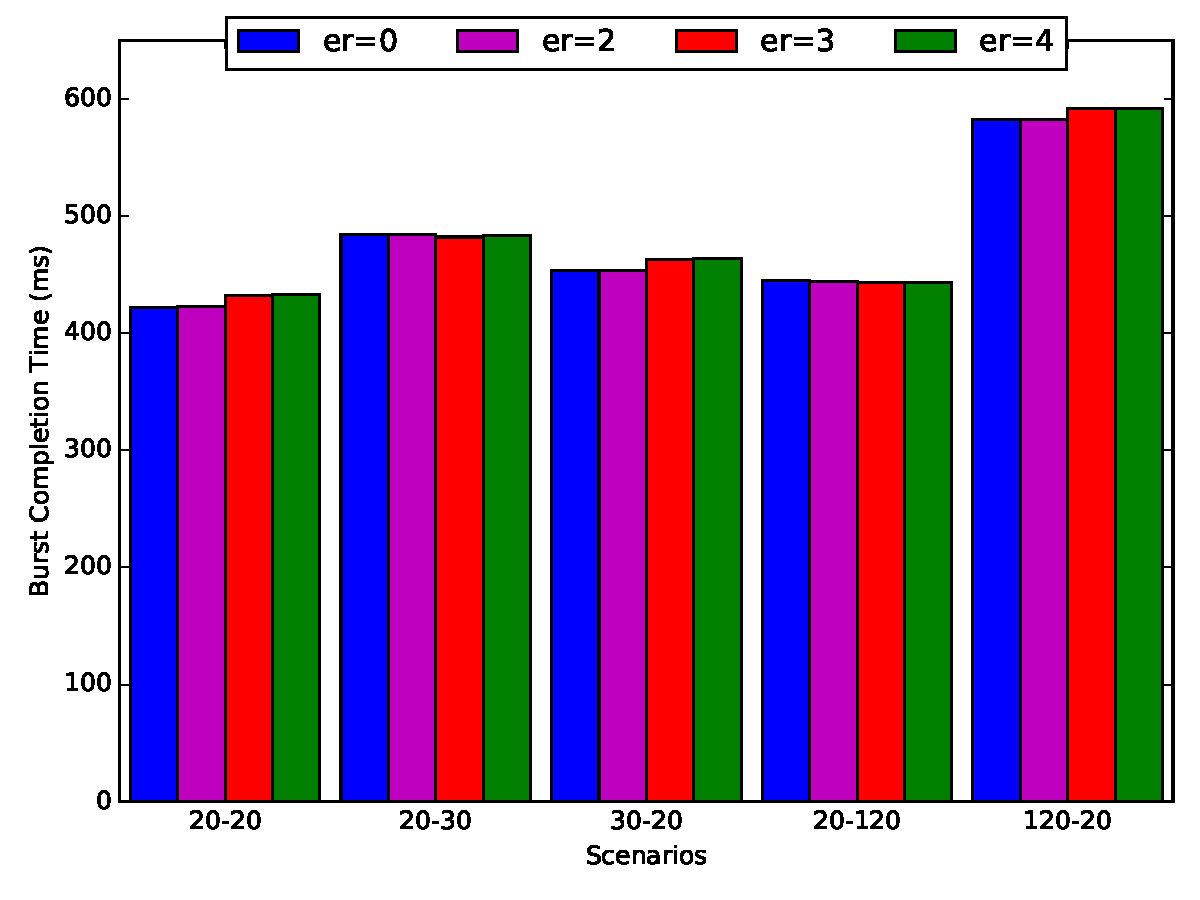
\includegraphics[angle=0, width=0.46\textwidth,natwidth=578.16,natheight=433.62]{plots/1P.pdf}
\caption{Single packet tail loss using MPTCP}\label{1p}
\end{center}
\end{figure}

In the case of single packet the last outstanding packet is sent as probe and in case of n-degree tail loss,
the latest packet is sent as probe to trigger fast retransmit of the packets in between. In order to observe
the performance of n-degree tail loss, we consider dropping the last two packets. 
The results of two packet tail loss are shown in Figure~\ref{2p}. In this case, TLP performs better than the other 
two settings in all scenarios except when the packets are lost on high delay interface. In this scenario, the delay difference is
large enough that the retransmission of last packet on alternate path is faster than the probe on the primary path. It 
is PTO time slower than the RTO setting.


\begin{figure}[!ht]
\begin{center}
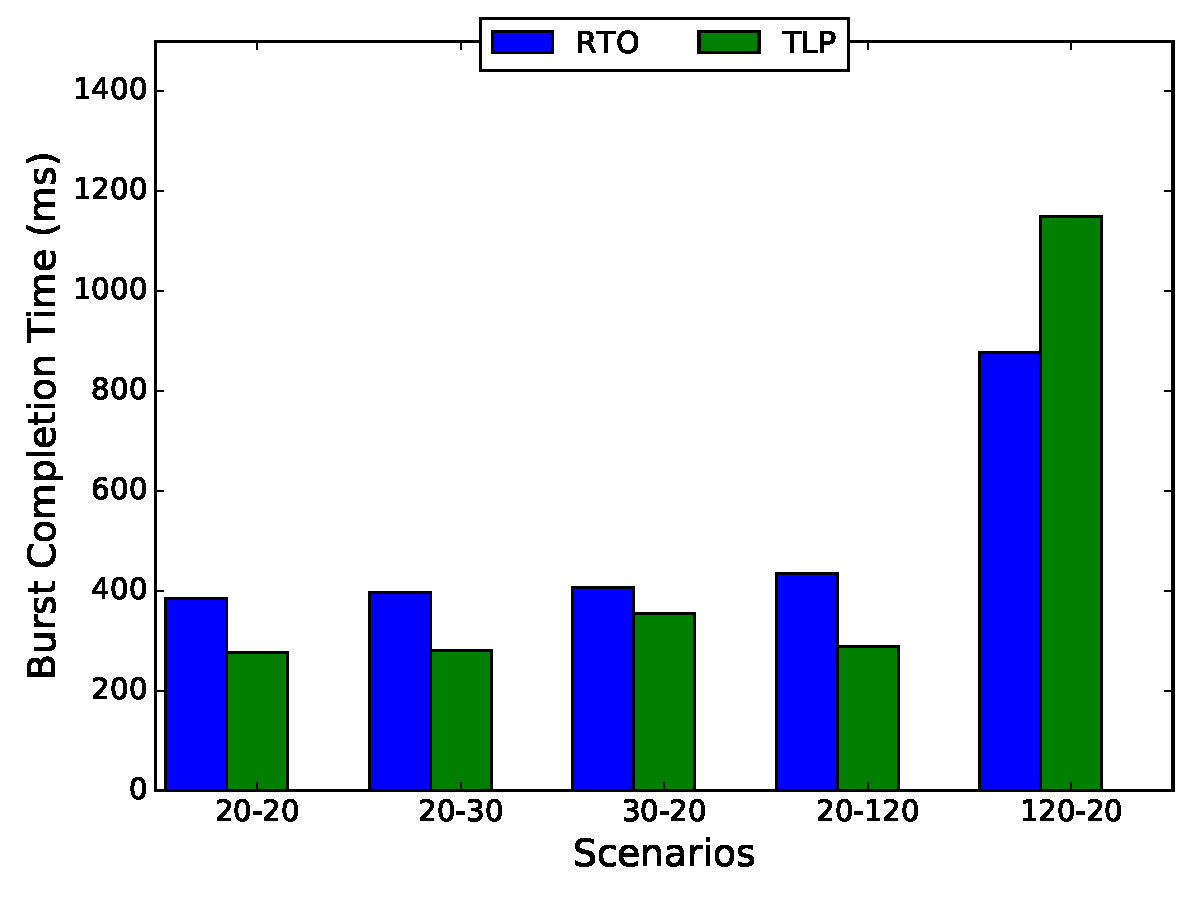
\includegraphics[angle=0, width=0.46\textwidth,natwidth=578.16,natheight=433.62]{plots/2P.pdf}
\caption{Two packet tail loss using MPTCP}\label{2p}
\end{center}
\end{figure}

To further study the performance of TLP in the case when there is longer path interruption on one path, we tried to drop the probe packet along with the last packet. In this scenario, the RTO
setting results in much lower burst completion times. Use of TLP did not improve the burst completion time as we saw in TCP for TLP. The reason
lies in the way the retransmission and loss probe transmission is carried out in MPTCP. Retransmission occurs after an RTO time on both paths.
Even if the retransmission fails on one path, the client receives the packet on the other path as shown in Fig~\ref{timing1P}. For TLP, in
current implementation, the loss probe is sent on the actual path of the first transmission but not on both paths. This incomplete impartation of
TLP from TCP to MPTCP led to the increase in burst completion time by an RTO for MPTCP. 


\begin{figure}[!ht]
\begin{center}
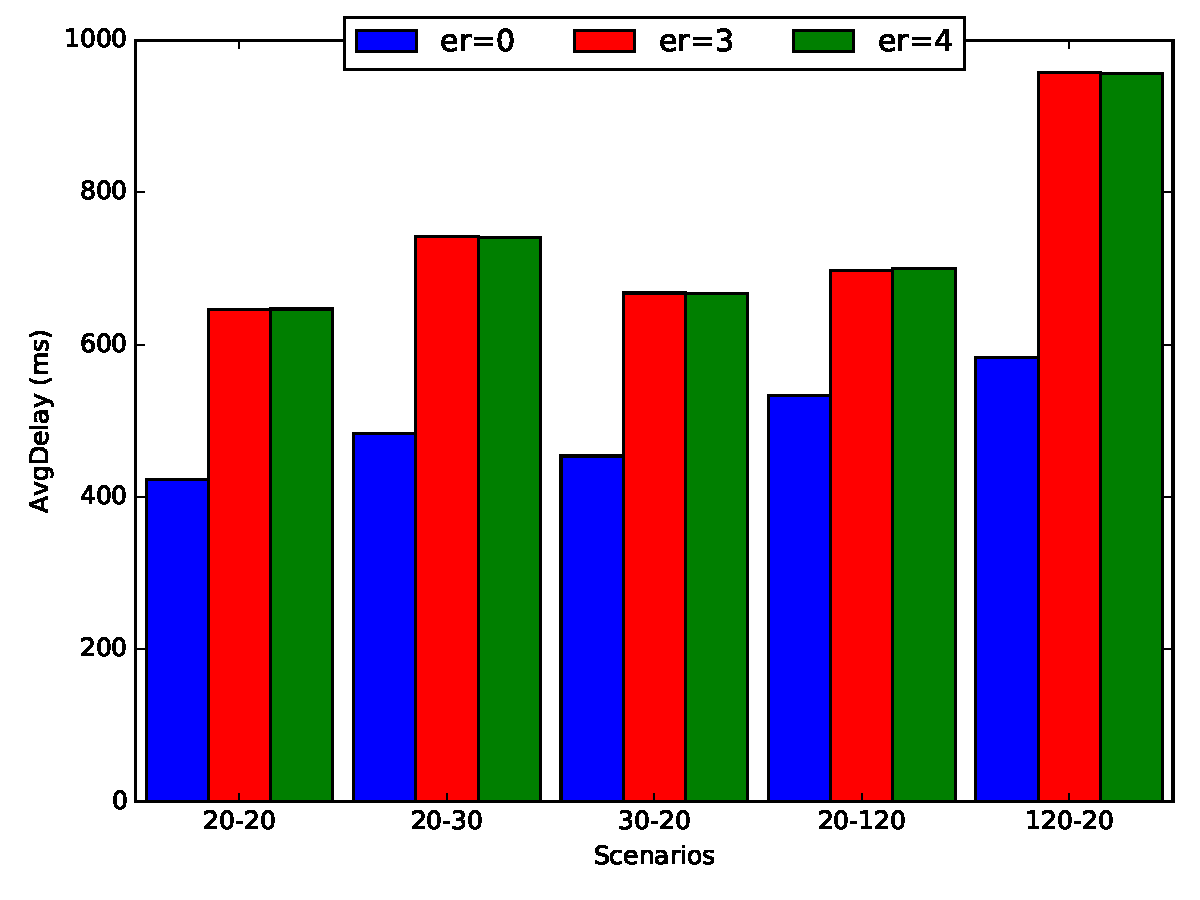
\includegraphics[angle=0, width=0.46\textwidth, natwidth=578.16,natheight=433.62]{plots/1PP.pdf}
\caption{Single packet tail loss together with probe loss using MPTCP}\label{1pp}
\end{center}
\end{figure}





%\begin{table}[!ht]
%\centering
%\caption{Tail loss scenarios with tcp.early.retrans = 3 default}
%\label{ret3}
%\begin{tabular}{|l|l|l|l|l|}
%\hline
% testcase   & Asymmetry   & Metalevel          & Subflowlevel       &  \\\hline
%Tail drop 1 & 20ms - 30ms & rexmt in same path & rexmt in same path &  \\\hline
%Tail drop 2 & 30ms - 20ms & rexmt in same path & TBC                &  \\\hline
%Tail drop 3 & 20ms - 20ms & rexmt in same path & TBC                &  \\ \hline
%\end{tabular}
%\end{table}





%\begin{table}[!ht]
%\centering
%\caption{Tail loss scenarios with tcp.early.retrans = 0 ER disabled}
%\label{ret0}
%\begin{tabular}{|l|l|l|l|l|}
%\hline
% testcase   & Asymmetry   & Metalevel          & Subflowlevel       &  \\\hline
%Tail drop 1 & 20ms - 30ms & rexmt in same path & rexmt in same path &  \\\hline
%Tail drop 2 & 30ms - 20ms & rexmt in same path & TBC                &  \\\hline
%Tail drop 3 & 20ms - 20ms & rexmt in same path & TBC                & \\ \hline
%Tail drop 4 & 20ms - 120ms &  			&		&  \\ \hline
%Tail drop 5 & 120ms - 20ms &  			& 		& \\ \hline 
%\end{tabular}
%\end{table}


%\begin{table}[!ht]
%\centering
%\caption{Tail loss scenarios with tcp.early.retrans = 4 TLP disabled}
%\label{ret4}
%\begin{tabular}{|l|l|l|l|l|}
%\hline
% testcase   & Asymmetry   & Metalevel          & Subflowlevel       &  \\\hline
%Tail drop 1 & 20ms - 30ms & rexmt in same path & rexmt in same path &  \\\hline
%Tail drop 2 & 30ms - 20ms & rexmt in same path & TBC                &  \\\hline
%Tail drop 3 & 20ms - 20ms & rexmt in same path & TBC                & \\ \hline
%\end{tabular}
%\end{table}


\section{Improvements to TLP for MPTCP}\label{impr}
The goal of Tail Loss Probe(TLP) is to reduce tail latency of short flows. It achieves this by converting retransmission timeouts (RTOs) occurring due to tail losses (losses at end of transactions) into fast recovery. TLP transmits one packet in two round-trips when a connection is in Open state and isn't receiving any ACKs. The transmitted packet, aka loss probe, can be either new or a retransmission. When there is tail loss, the ACK from a loss probe triggers FACK/early-retransmit based fast recovery, thus avoiding a costly retransmission timeout. Our results show that the current TLP implementation does not improve the performance in MPTCP in cases when there is path interruption and incur more latency.

The current implementation of TLP is at the TCP flow level. In the event of RTO timeout, the MPTCP retransmission happens with a re-injection in to the scheduler along with sending the lost packet on the same path. But in the event of Probe timeout, the loss probe packet is being sent on the same path without being re-injected in to the scheduler. We propose a modification to probe sending mechanism for MPTCP by re-injecting the probe packet in to the MPTCP scheduler in the event of PTO. As the probe timeout is meant for acting faster than the RTO timeout with essentially the same consequence as a retransmission, it is relevant to follow the same process as upon an RTO. It is expected that this modification is useful when the alternate path has lower delay than the packet original transmission path. The timing diagram depicted in Figure~\ref{timingNew} indicates the eventual behavior of modified MPTCP TLP for each of the studied loss. 

\begin{figure}[!ht]
\begin{center}
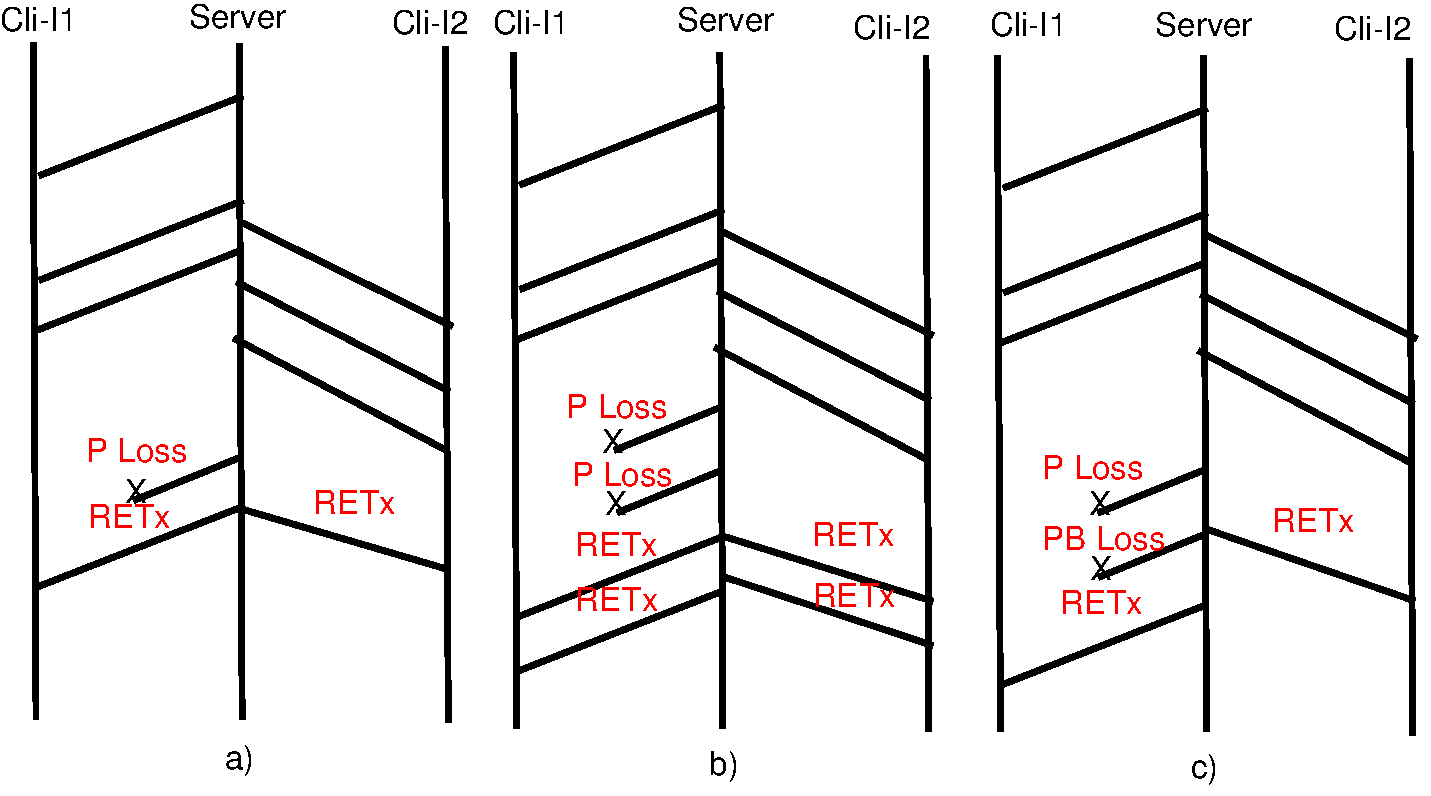
\includegraphics[angle=0, width=0.46\textwidth]{images/timingER3NewTLP.pdf}
\end{center}
\caption{Timing diagram of MPTCP behavior with proposed improvements with loss of a) One packet b) Two packet c) One packet and Retransmission}\label{timingNew}
\end{figure}


\section{Evaluation of modified MPTCP TLP}\label{eval}


Results comparing the burst completion time for new MPTCP TLP with that of TCP and MPTCP TLP for the considered cases are provided in Figures~\ref{1pn},~\ref{2pn} and ~\ref{1ppn}. 
In Figure~\ref{1pn}, MPTCP-New performs better than MPTCP in all scenarios, performs equal to TCP in symmetric scenarios and performs better than tcp in asymmetric scenarios. This improvement is due to RTO a packet to be retransmitted on the alternate path. In two packet tail loss scenario as in Figure~\ref{2pn}, MPTCP-New performs better than MPTCP in all scenarios and better than TCP in all scenarios except when the alternate path has higher delay than the original path. In the single packet together with probe loss scenario as in Figure~\ref{1ppn}, MPTCP-New performs better than both MPTCP and TCP in all scenarios with PTO triggering the probe retransmission on alternate path much earlier than the RTO.


\begin{figure}[!ht]
\begin{center}
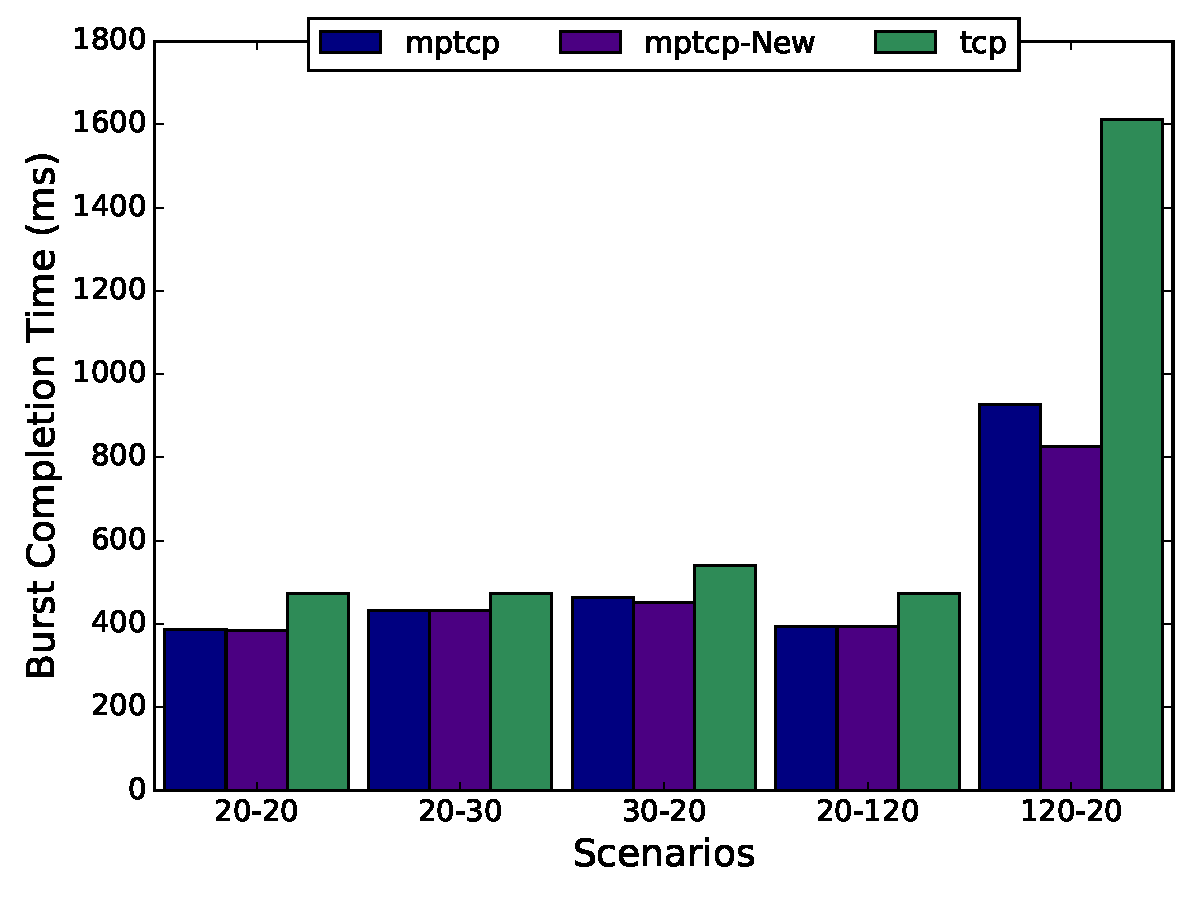
\includegraphics[angle=0, width=0.46\textwidth, natwidth=578.16,natheight=433.62]{plots/1PNew.pdf}
\caption{Single packet tail loss comparison with MPTCP, TCP}\label{1pn}
\end{center}
\end{figure}

\begin{figure}[!ht]
\begin{center}
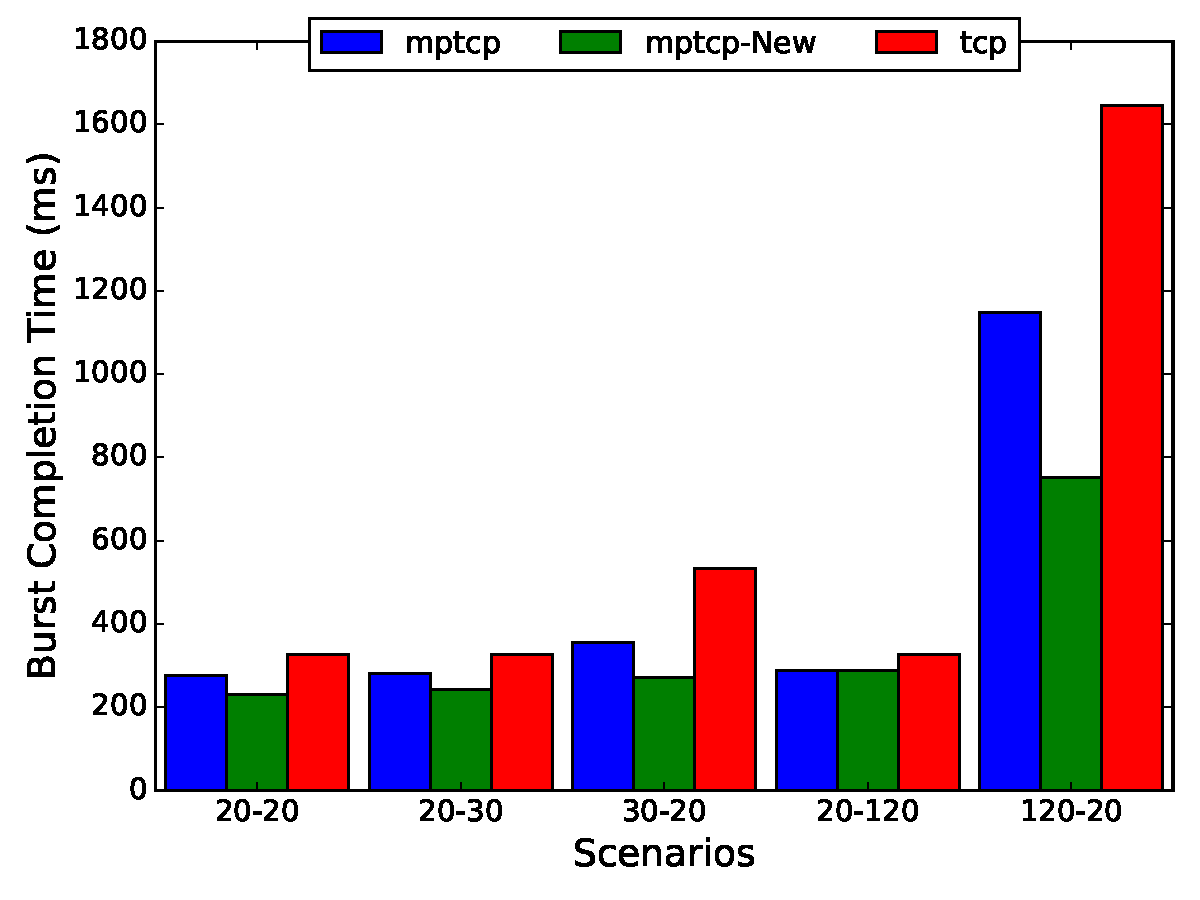
\includegraphics[angle=0, width=0.46\textwidth, natwidth=578.16,natheight=433.62]{plots/2PNew.pdf}
\caption{Two packet tail loss comparison with MPTCP, TCP}\label{2pn}
\end{center}
\end{figure}

\begin{figure}[!ht]
\begin{center}
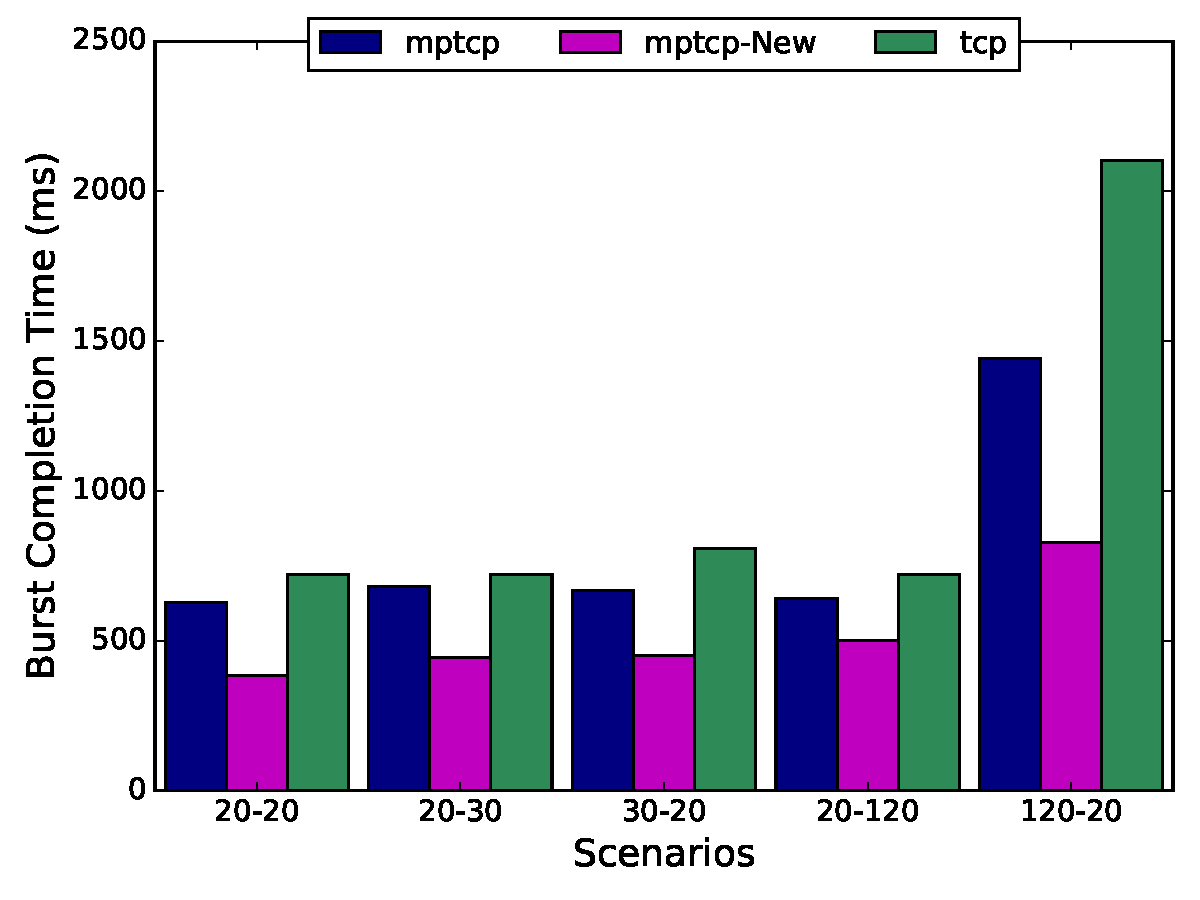
\includegraphics[angle=0, width=0.46\textwidth, natwidth=578.16,natheight=433.62]{plots/1PPNew.pdf}
\caption{Single packet tail loss together with probe loss with MPTCP, TCP}\label{1ppn}
\end{center}
\end{figure}


\section{Conclusion}\label{conc}
This paper provides the short comparative analysis of retransmission behavior with TCP and MPTCP protocols using various loss patterns for tail losses.
The three cases of tail losses together with deterministic loss pattern allow us to dissect the retransmission behavior at packet level to understand possible improvements.
We propose a less conservative approach to trigger retransmission on an alternate path in the event of tail loss probe timeout, which otherwise triggered with an RTO. 
Our emulation experiments  using a modified Linux implementation, show that the proposed approach in fact improves the burst completion time in most cases and equals the existing
implementation in other cases. The proposed approach improves the performance when the alternate path has lower delay than the original loss path and the advantage increases with degree of asymmetry between the paths. Temporary path failures can cause probe loss along with packet loss. The approach is very effective in case of probe loss which otherwise incur RTO timeout to trigger retransmission on either path. However, the latency improvement comes at a cost of additional network traffic from the retransmitted packets. Further, we plan to investigate more conservative approaches for other retransmission events.    
   
\bibliographystyle{IEEEtran}
\bibliography{mptcp-retrans}
\end{document} 
